\graphicspath{{images/agreement/}}

\section{Договоры}
Платформа позволяет реализовать следующий сценарий: на Платформе создаются университеты, администраторы добавляют курсы, которые привязываются к разработавшему их вузу. В дальнейшем университеты могут заключать между собой договоры на покупку права обучать студентов одного университета на курсах другого в течение периода времени, установленного договором. В этом случае университет, предоставляющий свои курсы называется вузом"=разработчиком (поставщиком), университет, осуществляющий покупку, "--- вузом-потребителем (потребителем). Один и тот же университет может выступать как поставщик в одних договорах и как потребитель в других.

Раздел \quotes{Договоры} предоставляет средства для организации этапов описанного выше сценария.

Краткое описание состава раздела:
\begin{itemize}
	\item \textbf{Функции поставщика}
	\begin{itemize}
		\item \textbf{Договоры на предоставление услуг.} Подраздел выводит информацию о договорах, в которых данный университет является поставщиком. Из этого подраздела осуществляется переход к подразделам:
		\begin{itemize}
			\item \textbf{Просмотр информации о договоре.} Предоставляет подробную информацию о договоре.
			\item \textbf{Редактирование договора.} Предоставляет поставщику возможность редактирования созданного договора
		\end{itemize}
		\item \textbf{Платежи.} Платежи слушателей курса за прохождение курса.
		\item \textbf{Заявки на зачисление.} Вузы"=потребители могут подавать заявки на зачисление своих студентов, перечисленных в заявке, на курсы вуза"=разработчика. В этом подразделе выводится информация о заявках, поступивших данному университету, как поставщику.  Из этого подраздела осуществляется переход к подразделу:
		\begin{itemize}
			\item \textbf{Просмотр информации и управление статусом заявки.} Предоставляет подробную информацию о заявке. В этом подразделе поставщик может принять или отклонить поступившую заявку.
		\end{itemize}
		\item \textbf{Заявки на изменение режима прохождения сессии курса.} Для сессии курса может существовать несколько режимов прохождения (подробнее см. раздел \quotes{Курсы}), вуз"=потребитель может подавать заявки на изменение режима прохождения сессии для группы своих студентов из числа зачисленных, которая указана в заявке. В этом подразделе выводится информация о заявках на изменении режима прохождения сессии, поступивших данному университету, как поставщику. Из этого подраздела осуществляется переход к подразделу:
		\begin{itemize}
			\item \textbf{Просмотр информации и управление статусом заявки.} Предоставляет подробную информацию о заявке. В этом подразделе поставщик может принять или отклонить поступившую заявку.
		\end{itemize}
		\item \textbf{Добавить договор.} Подраздел предоставляет поставщику возможность создания договора на предоставление своих курсов.
	\end{itemize}
	
	\item \textbf{Функции потребителя}
	\begin{itemize}
		\item \textbf{Договоры на получение услуг.} Подраздел выводит информацию о договорах, в которых данный университет является потребителем. Из этого подраздела осуществляется переход к подразделу
		\begin{itemize}
			\item \textbf{Просмотр информации о договоре.} Предоставляет подробную информацию о договоре.
		\end{itemize}
	\end{itemize}
\end{itemize}

Навигация по компонентам раздела осуществляется с помощью левой панели вспомогательного меню, структура которого соответствует описанному выше составу раздела.

\subsection{Роли и операции}
Раздел доступен пользователям, имеющим следующие роли:	
	\begin{itemize}
		\item Администратор Платформы:
		\begin{itemize}
			\item просмотр договоров на предоставление услуг;
			\item просмотр подробной информации о договорах на предоставление услуг;
			\item редактирование договоров;
			\item просмотр платежей;
			\item просмотр заявок на зачисление и управление статусом заявок;
			\item просмотр заявок на изменение режима прохождения сессий и управление статусом заявок;
			\item создание договоров.
		\end{itemize}
		\item Администратор вуза"=поставщика:
		\begin{itemize}
			\item просмотр договоров на предоставление услуг;
			\item просмотр подробной информации о договорах на предоставление услуг;
			\item редактирование договоров;
			\item просмотр платежей;
			\item просмотр заявок на зачисление и управление статусом заявок;
			\item просмотр заявок на изменение режима прохождения сессий и управление статусом заявок;
			\item создание договоров.
		\end{itemize}
		\item Автор курса:
		\begin{itemize}
			\item просмотр договоров на предоставление услуг (притом выводится информация только по тем договорам, в которых участвуют курсы, автором которых является данный пользователь);
			\item просмотр подробной информации о договорах на предоставление услуг(имеются в виду те договоры, в которых участвуют курсы, автором которых является данный пользователь).
		\end{itemize}				
		\item Администратор вуза"=потребителя:
		\begin{itemize}
			\item просмотр договоров на получение услуг;
			\item просмотр подробной информации о договорах на получение услуг.
		\end{itemize}				
	\end{itemize} 
	
	\subsection{Договоры на предоставление услуг}\label{agreement:provider_agreements_section}
При выборе в главном меню пункта \quotes{Договоры} осуществляется переход в подраздел \quotes{Договоры на предоставление услуг}, если роль пользователя позволяет просматривать этот подраздел.
Подраздел предоставляет информацию о договорах, в которых данный вуз выступает в роли поставщика. Информация представлена в виде таблицы, строки которой соответствуют договорам. Внешний вид раздела  приведён на рисунке~\ref{agreement:provider_agreements}
	
	\begin{figure}[H]
	\center{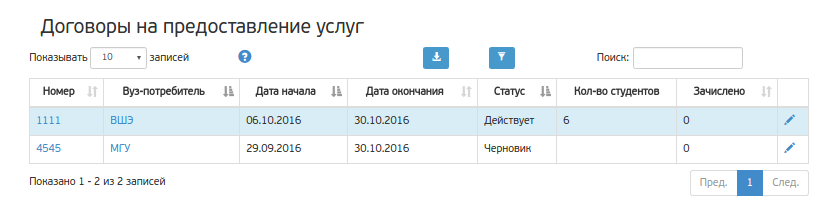
\includegraphics[width=1\linewidth]{provider_agreements.png}}
	\caption{Внешний вид подраздела \quotes{Просмотр договоров на предоставление услуг}}
	\label{agreement:provider_agreements}
	\end{figure}
	
\textbf{Перечень столбцов таблицы:}
\begin{itemize}
	\item \textbf{Номер.} Номер договора является ссылкой, по нажатию осуществляется переход к подразделу \quotes{Просмотр подробной информации о договоре}.
	\item \textbf{Вуз"=потребитель.} Аббревиатура вуза"=потребителя, с которым заключен данный договор, является ссылкой, по нажатию осуществляется переход на станицу университета на сайте.
	\item \textbf{Дата начала.} Дата начала договора.
	\item \textbf{Дата окончания.} Дата окончания договора.
	\item \textbf{Статус.} Статус договора принимает одно из трех возможных значений: \quotes{Черновик},  \quotes{Действует},  \quotes{Не действует}. Создание заявок на зачисление на стороне потребителя возможно только по действующему договору. Договоры, имеющие статус  \quotes{Черновик} и \quotes{Не действует} не показываются потребителям в соответствующем разделе \quotes{Договоры на получение услуг}.
	\item \textbf{Количество студентов.} При создании/редактировании договора можно указывать максимальное количество студентов для каждого курса, которые могут быть зачислены по данному договору. Количество студентов "--- суммарное максимальное количество студентов по всем курсам, указанным в договоре, может быть не указано.
	\item \textbf{Зачислено.} Фактическое суммарное количество зачисленных студентов по данному договору на текущий момент.
	\item \textbf{Иконка редактирования.} По нажатию осуществляется переход в подраздел \quotes{Редактирование договора}, скрывается в случае, если роль пользователя не позволяет редактировать договоры.
\end{itemize}

\subsubsection{Элементы управления}
Помимо общих элементов управления табличными данными, описанных в подразделе~\ref{sec:datatables}, на странице раздела присутствует 
иконка \quotes{Справка} \vcenteredinclude[height=25px]{table_help.png}, которая выводит справочную информацию о таблице. 
При нажатии появляется всплывающее окно, в котором описан принцип подсветки фона строк таблицы: 
цвет фона строки отличается в зависимости от наличия и статуса заявок на зачисление студентов по договору, 
которому соответствует  данная строка (см. рис.~\ref{agreement:table_help_legend}).
	
\begin{figure}[H]
\center{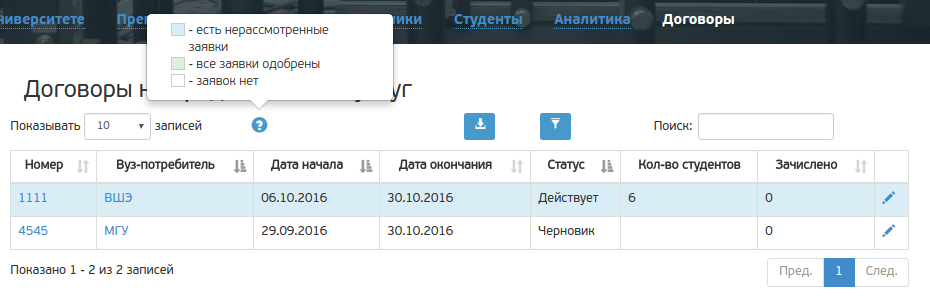
\includegraphics[width=1\linewidth]{table_help_legend.png}}
\caption{Всплывающее окно с подсказкой}
\label{agreement:table_help_legend}
\end{figure}	

Форма фильтрации в данном подразделе позволяет задавать следующие параметры:
\begin{itemize}
	\item университет - позволяет выбрать одного или нескольких вузов-потребителей, принципы работы с полями такого типа описаны в подразделе ~\ref{widget:autocomplete_with_multiselect};
	\item статус договора;
	\item дата начала договора от (принципы работы с полями такого типа описаны в подразделе ~\ref{widget:date_time_picker});
	\item дата начала договора до (принципы работы с полями такого типа описаны в подразделе ~\ref{widget:date_time_picker});
	\item дата окончания договора от (принципы работы с полями такого типа описаны в подразделе ~\ref{widget:date_time_picker});
	\item дата окончания договора до (принципы работы с полями такого типа описаны в подразделе ~\ref{widget:date_time_picker});
	\item заявки - позволяет отфильтровать договоры в соответствии с наличием и статусом заявок, принципы работы с полями такого типа описаны в подразделе ~\ref{widget:autocomplete_with_multiselect};
\end{itemize}

\subsection{Договоры на получение услуг}
Переход в данный подраздел осуществляется по выбору соответствующего пункта вспомогательного меню на панели, расположенной слева.

Данный подраздел предоставляет информацию о договорах, в которых данный вуз является потребителем, причем отображается только информация по договорам в статусе \quotes{Действует}.

Возможность доступа к подразделу имеется только у администратора вуза"=потребителя.

Содержание подраздела, возможные действия и реакции полностью аналогичны описанным в подразделе~\ref{agreement:provider_agreements_section} за исключением двух моментов:
\begin{itemize}
	\item В таблице, содержащей информацию о договорах отсутствует колонка с иконкой для переход к подразделу  \quotes{Редактирование договора}, так как администратор вуза"=потребителя не имеет права на редактирование договоров.
	\item В таблице, содержащей информацию о договорах отсутствует колонка \quotes{Статус}, так как в данном разделе выводится информация только о действующих договорах. Договоры в статусе \quotes{Черновик} и \quotes{Не действует}, заключенные с данным вузом"=потребителем, видны только из кабинетов поставщиков, заключивших эти договоры.
	\item В таблице, содержащей информацию о договорах, вместо колонки \quotes{Вуз-потребитель} добавлена колонка \quotes{Вуз-разработчик}, содержащая аббревиатуру вуза-разработчика в договоре, является ссылкой на страницу университета на сайте.
\end{itemize}


\subsection{Просмотр подробной информации по договору}
Позволяет просмотреть подробную  информацию по интересующему договору. Информацию по заключенному договору доступна для просмотра как поставщику, так и потребителю, однако, для последнего она выводится в ограниченном виде.
Администратор Платформы может просматривать полную информацию обо всех договорах.

Администратор вуза"=поставщика может просматривать полную информацию по всем договорам, в которых вуз выступает в роли поставщика.

Администратор  вуза"=потребителя может просматривать ограниченную информацию по действующим договорам, в которых вуз является поставщиком.

Автор курса может просматривать ограниченную информацию о договорах, в которых фигурируют курсы, автором которых он является.

Перейти в раздел можно, нажав на номер договора в таблице в разделе \quotes{Просмотр договоров на предоставление услуг} (просмотр в роли поставщика), или в разделе \quotes{Просмотр договоров на получение услуг} (просмотр в роли потребителя). Внешний вид подраздела приведён на рисунке~\ref{agreement:detailview}
	
	\begin{figure}[H]
	\center{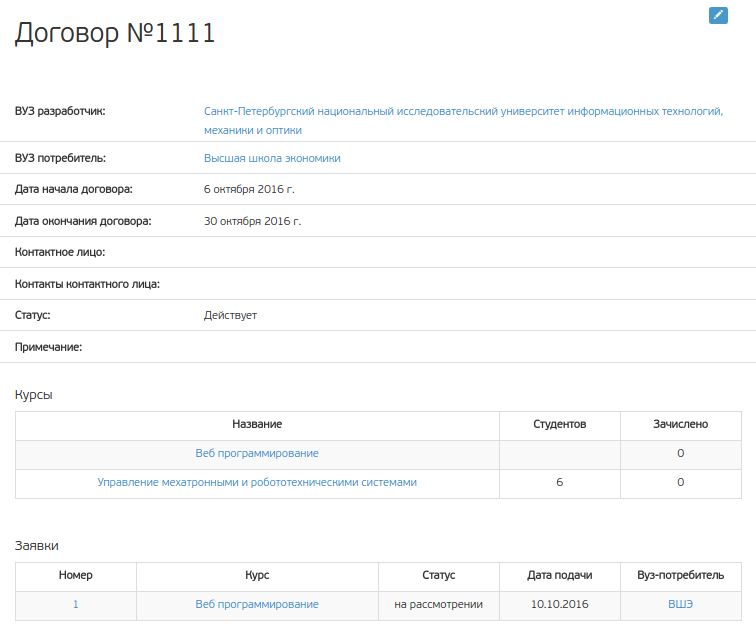
\includegraphics[width=1\linewidth]{detailview.png}}
	\caption{Просмотр подробной информации о договоре}
	\label{agreement:detailview}
	\end{figure}

Набор доступных для просмотра полей отличается в зависимости от роли пользователя: Администратору Платформы и администратору вуза"=поставщика доступны все поля, перечисленные ниже; администратору вуза"=потребителя и автору курса доступны только поля выделенные жирным шрифтом:
\begin{itemize}
	\item \textbf{Номер договора.} Указан в заголовке.
	\item \textbf{Вуз разработчик.} Название вуза, который выполняет роль поставщика в данном договоре. Является ссылкой, по нажатию осуществляется переход на страницу университета на сайте.
	\item \textbf{Вуз потребитель.} Название вуза, который выполняет роль потребителя в данном договоре. Яявляется ссылкой, по нажатию осуществляется переход на страницу университета на сайте.
	\item \textbf{Дата начала договора.}
	\item \textbf{Дата окончания договора.}
	\item \textbf{Контактное лицо.} Контактное лицо со стороны вуза"=потребителя для связи по данному договору.
	\item \textbf{Контакты контактного лица.} Контакты (e"=mail, номер телефона, др.) контактного лица со стороны вуза"=потребителя для связи по данному договору.
	\item Статус договора принимает одно из трех возможных значений: \quotes{Черновик},  \quotes{Действует},  \quotes{Не действует}. Создание заявок на зачисление на стороне потребителя возможно только по действующему договору. Договоры, имеющие статус  \quotes{Черновик} и \quotes{Не действует} не показываются потребителям в соответствующем разделе \quotes{Договоры на получение услуг}.
	\item Примечание. Любое примечание поставщика.
	\item \textbf{Курсы.} Информация о курсах, заявленных в данном договоре, представлена в виде таблицы.
	\item Заявки. Информация о заявках на зачисление студентов по данному договору, если таковые имеются, представлена в виде таблицы.
\end{itemize}

\subsubsection{Элементы управления}
В данном разделе имеется один элемент управления "--- иконка \quotes{Редактировать} \vcenteredinclude[width=0.1\linewidth]{edit_icon.png}, которая видна в том случае, если роль пользователя предоставляет право редактирования договора.


\subsection{Редактирование договора}\label{agreement:edit_section}
Переход в подраздел осуществляется по нажатию иконки \quotes{Редактировать} \vcenteredinclude[width=0.1\linewidth]{edit_icon.png} в строке таблицы, соответствующей редактируемому  договору в подразделе \quotes{Договоры на предоставление услуг}, или в подразделе \quotes{Просмотр подробной информации о договоре}.

Подраздел предоставляет возможность изменять значения полей:
\begin{itemize}
	\item Номер договора;
	\item Дата начала договора;
	\item Дата окончания договора;
	\item Контактное лицо со стороны вуза"=потребителя для связи по данному договору;
	\item Контакты контактного лица. Контакты (e"=mail, номер телефона, др.) контактного лица со стороны вуза"=потребителя для связи по данному договору;
	\item Статус договора принимает одно из трех возможных значений: \quotes{Черновик},  \quotes{Действует},  \quotes{Не действует}. Создание заявок на зачисление на стороне потребителя возможно только по действующему договору. Договоры, имеющие статус  \quotes{Черновик} и \quotes{Не действует} не показываются потребителям в соответствующем разделе \quotes{Договоры на получение услуг};
	\item Примечание;
	\item Курсы, на которые заключается договор.
\end{itemize}

\subsubsection{Поля и ошибки}
В форме представлено несколько типов полей:
	\begin{itemize}
		\item \textbf{Обязательные поля} отмечены символом \quotes{*}, если такое поле оставить не заполненным "--- появляется сообщение о необходимости его заполнения и блокируется кнопка сохранения изменений (см. рис.~\ref{agreement:edit_required}).
		
		\begin{figure}[H]
		\center{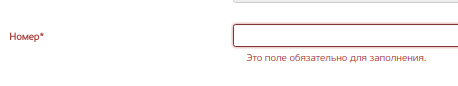
\includegraphics[width=1\linewidth]{edit_required.png}}
		\caption{Обработка заполнения обязательных полей}
		\label{agreement:edit_required}
		\end{figure}	
		
		\item \textbf{Даты начала и окончания договора.} "--- виджет выбора даты, подробно описанный в подразделе~\ref{widget:date_time_picker};
		\item \textbf{Курсы.} Данный элемент формы представляет собой подраздел, в котором происходит редактирование курсов, на которые заключается договор. Каждый курс представлен в этой области строкой, которая включает в себя элементы:
		\begin{itemize}
			\item Название курса. Выбор происходит из выпадающего списка.
			\item Количество студентов. Максимальное количество студентов, которое планируется зачислить по данному курсу в рамках договора, при превышении этого количества на этапе принятия/отклонения заявок на зачисление администратор вуза"=поставщика, будет получать предупреждения.
			\item Зачислено. Фактическое количество зачисленных студентов по данному курсу в рамках договора на текущий момент.
		\end{itemize}
		Внешний вид области редактирования курсов представлен на рисунке~\ref{agreement:edit_course}.
		\begin{figure}[H]
		\center{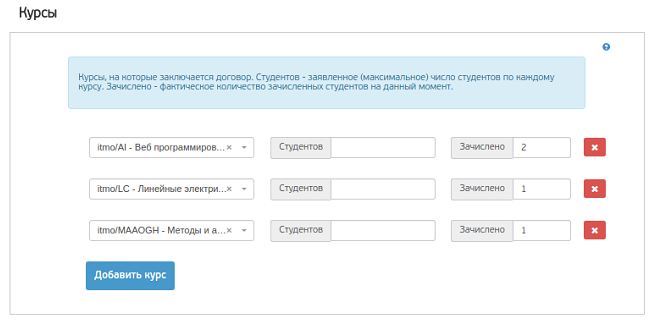
\includegraphics[width=1\linewidth]{edit_course.png}}
		\caption{Внешний вид области редактирования курсов}
		\label{agreement:edit_course}
		\end{figure}	
		
		Для того, чтобы добавить курс к договору необходимо нажать на кнопку \quotes{Добавить}(см. рис.~\ref{agreement:edit_course_add}). В появившейся строке можно выбрать курс из числа курсов, предоставляемых данным вузом. Один и тот же курс может быть добавлен к договору не больше одного раза. Подробная информация о работе с полями, содержащими виджет выпадающего списка с автодополнением доступна в разделе~\ref{widget:autocomplete}. Поле \quotes{Курс} является обязательным для заполнения, если попробовать сохранить формы с добавленной, но не заполненной строкой курса, появится сообщение об ошибке (см. рис.~\ref{agreement:edit_course_required}).
		
		\begin{figure}[H]
		\center{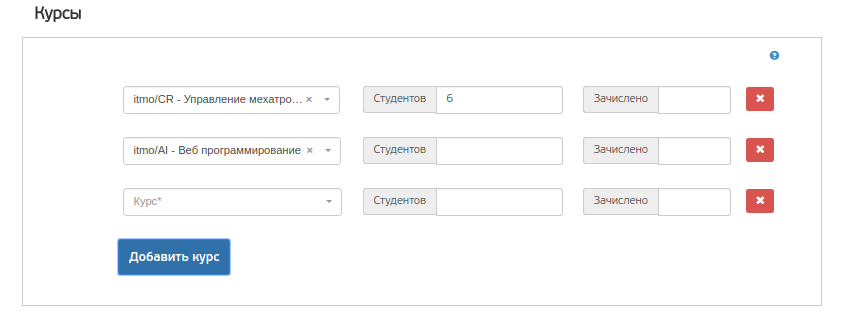
\includegraphics[width=1\linewidth]{edit_course_add.png}}
		\caption{Добавление курса к договору}
		\label{agreement:edit_course_add}
		\end{figure}	
		
		\begin{figure}[H]
		\center{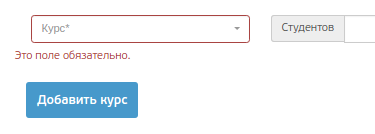
\includegraphics[height=3cm]{edit_course_required.png}}
		\caption{Ошибка сохранения формы с незаполненным полем курса}
		\label{agreement:edit_course_required}
		\end{figure}	
		
Для удаления курса из договора необходимо нажать на иконку \quotes{Удалить} \vcenteredinclude[width=0.1\linewidth]{edit_course_delete.png}. 
Если на момент удаления по данному курсу нет зачисленных студентов или заявок в статусе \quotes{на рассмотрении}, курс будет удален из договора. 
В противном случае появится окно с предупреждением о наличии студентов/заявок (см. рис.~\ref{agreement:edit_course_warn}).
	\begin{figure}[H]
		\center{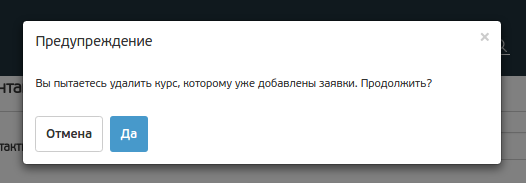
\includegraphics[width=1\linewidth]{edit_course_warn.png}}
		\caption{Предупреждение о наличии заявок по удаляемому курсу}
		\label{agreement:edit_course_warn}
	\end{figure}	
Если нажать \quotes{Ок} "--- курс будет удален из договора. Если нажать \quotes{Отмена} или кликнуть за пределы окна с предупреждением, процесс удаления будет остановлен.

Если указанное значение количества студентов в договоре меньше, чем количество уже зачисленных студентов по этому договору, 
при сохранении формы появится окно с предупреждением (см. рис.~\ref{agreement:edit_course_warn_number}).

		\begin{figure}[H]
		\center{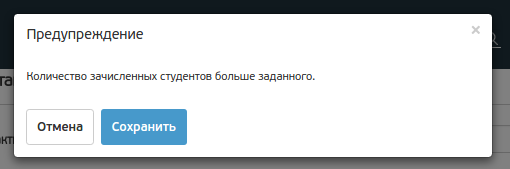
\includegraphics[width=1\linewidth]{edit_course_warn_number.png}}
		\caption{Предупреждении о превышении максимального количества студентов}
		\label{agreement:edit_course_warn_number}
		\end{figure}
		
Если нажать \quotes{Ок} "--- форма будет сохранена, в случае нажатия кнопки \quotes{Отмена} или клику за пределы окна с предупреждением, процесс сохранения изменений будет остановлен, поле, в котором произошло превышение, будет подсвечено красным (см рис.~\ref{agreement:edit_course_warn_cancel}).	

		\begin{figure}[H]
		\center{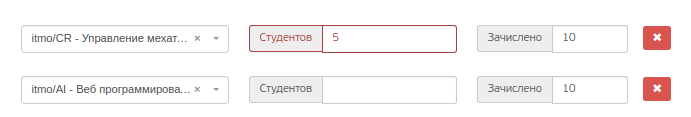
\includegraphics[width=1\linewidth]{edit_course_warn_cancel.png}}
		\caption{Предупреждении о превышении максимального количества студентов}
		\label{agreement:edit_course_warn_cancel}
		\end{figure}
			
При удалении всех курсов из договора и попытке сохранения договора, появится сообщение об ошибке (см. рис.~\ref{agreement:edit_course_nothing}).
	
		\begin{figure}[H]
		\center{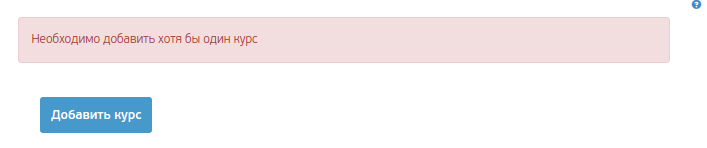
\includegraphics[width=1\linewidth]{edit_course_nothing.png}}
		\caption{Ошибка сохранения договора без курсов}
		\label{agreement:edit_course_nothing}
		\end{figure}

 	\end{itemize}
 	
\subsubsection{Элементы управления}
Управление внесенными изменениями осуществляется с помощью кнопок расположенных внизу страницы (см. рис.~\ref{agreement:edit_buttons}).
		\begin{figure}[H]
		\center{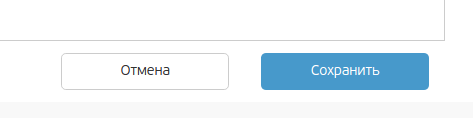
\includegraphics[width=1\linewidth]{edit_buttons.png}}
		\caption{Элементы управления подраздела \quotes{Редактирование договора}}
		\label{agreement:edit_buttons}
		\end{figure}	
		
При нажатии \quotes{сохранить} осуществляется попытка сохранения формы. 
Если форма заполнена корректно, то внесенные изменения сохраняются, а пользователь перенаправляется в раздел \quotes{Просмотр подробной информации о договоре}.
Если имеются ошибки "--- отображаются сообщения об ошибках, осуществляется прокрутка к месту первой ошибки. 

При нажатии кнопки \quotes{отмена} все изменения теряются, пользователь перенаправляется на предыдущую страницу.


\subsection{Создание договора}
Подраздел позволяет администратору вуза"=поставщика создать договор на предоставление услуг вузу"=потребителю.

Переход в подраздел осуществляется по выбору соответствующего пункта вспомогательного меню, расположенного на левой панели.

Форма создания, ее состав, возможные действия и реакции аналогичны описанным в разделе~\ref{agreement:edit_section}, за исключение нескольких отличий:
\begin{itemize}
	\item При создании договора заполняется поле \quotes{Вуз"=потребитель} (подробная информация о работе с полями, содержащими виджет выпадающего списка с автодополнением доступна в разделе~\ref{widget:autocomplete}), которое нельзя изменить после сохранения договора. Это поле является обязательным. После выбора потребителя поля \quotes{Контактное лицо} и \quotes{Контакты контактного лица} заполняются значениями по умолчанию, указанными в описании вуза"=потребителя. 
	При желании создатель договора может отредактировать эти поля по собственному усмотрению.
	\item В области добавления курсов отсутствует графа \quotes{Зачислено}, так как при создании нового договора никаких зачислений по нему быть не может.
\end{itemize}

\subsection{Платежи}
Данный подраздел предоставляет информацию о платежах.

Переход в подраздел осуществляется по выбору соответствующего пункта вспомогательного меню, расположенного на левой панели.

Информация о платежах представлена в виде таблицы, каждая строка которой соответствует конкретному платежу. 
Таблица имеет следующие колонки:
\begin{itemize}
	\item Дата создания платежа.
	\item Студент, который осуществляет платеж.
	\item Сумма, на которую осуществляется платеж.
	\item Номер заказа.
	\item Статус платежа. Возможны следующие значения: \quotes{Processed}, \quotes{Success}, \quotes{Fail}.
	\item Дата платежа. Дата, соответствующая моменту, когда платеж произведен.
\end{itemize}

Внешний вид раздела представлен на рисунке~\ref{agreement:table_payments}.
		\begin{figure}[H]
		\center{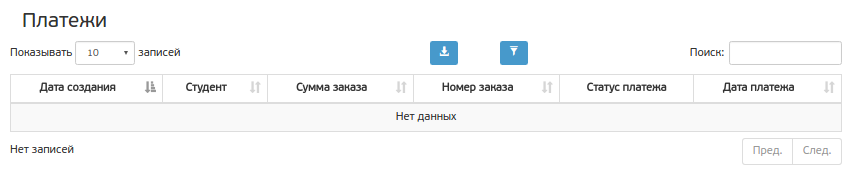
\includegraphics[width=1\linewidth]{table_payments.png}}
		\caption{Внешний вид подраздела \quotes{Платежи}}
		\label{agreement:table_payments}
		\end{figure}	
		
\subsubsection{Элементы управления}
Элементы управления табличными представления описаны в подразделе~\ref{sec:datatables}. Вид формы фильтрации приведён на рисунке~\ref{agreement:payments_filter_form}
\begin{figure}[H]
	\center{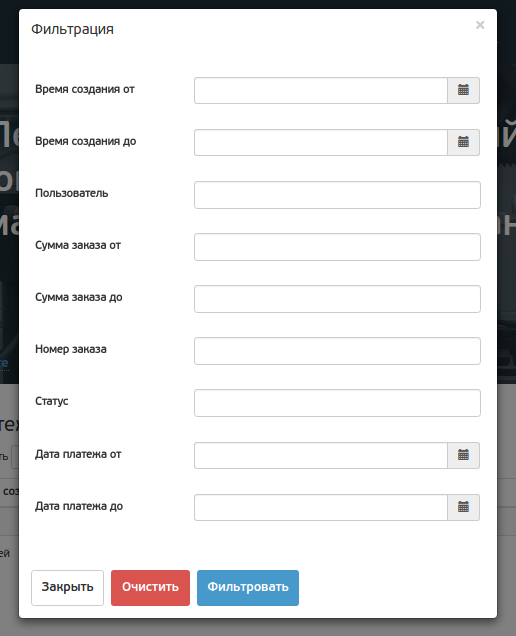
\includegraphics[height=10.5cm]{payments_filter_form.png}}
	\caption{Вид формы фильтрации для подраздела \quotes{Платежи}}
	\label{agreement:payments_filter_form}
\end{figure}

Можно фильтровать список по следующим параметрам:
\begin{itemize}
	\item Диапазон дат создания "--- виджеты выбора даты и времени 
	(описание виджета см. в подразделе~\ref{widget:date_time_picker});
	\item Пользователь "--- виджет выпадающего списка с автодополнением с возможностью множественного выбора 
	(описание виджета см. в подразделе~\ref{widget:autocomplete_with_multiselect});
	\item Диапазон суммы заказа "--- числовое поле.
	\item Номер заказа "--- текстовое поле.
	\item Статус "--- виджет выпадающего списка с автодополнением с возможностью множественного выбора 
	(описание виджета см. в подразделе~\ref{widget:autocomplete_with_multiselect});
	\item Диапазон дат платежа "--- виджеты выбора даты и времени.
\end{itemize}


\subsection{Заявки на зачисление студентов}

Заявки на зачисление "--- это табличное представление заявок на зачисление студентов, 
полученных данным вузом в качестве вуза-разработчика. 
Элементы управления табличными представления описаны в подразделе~\ref{sec:datatables}.
Внешний вид списка представлен на рис.~\ref{img:agreement:enroll_req_list}. 

\begin{figure}[H]
	\center{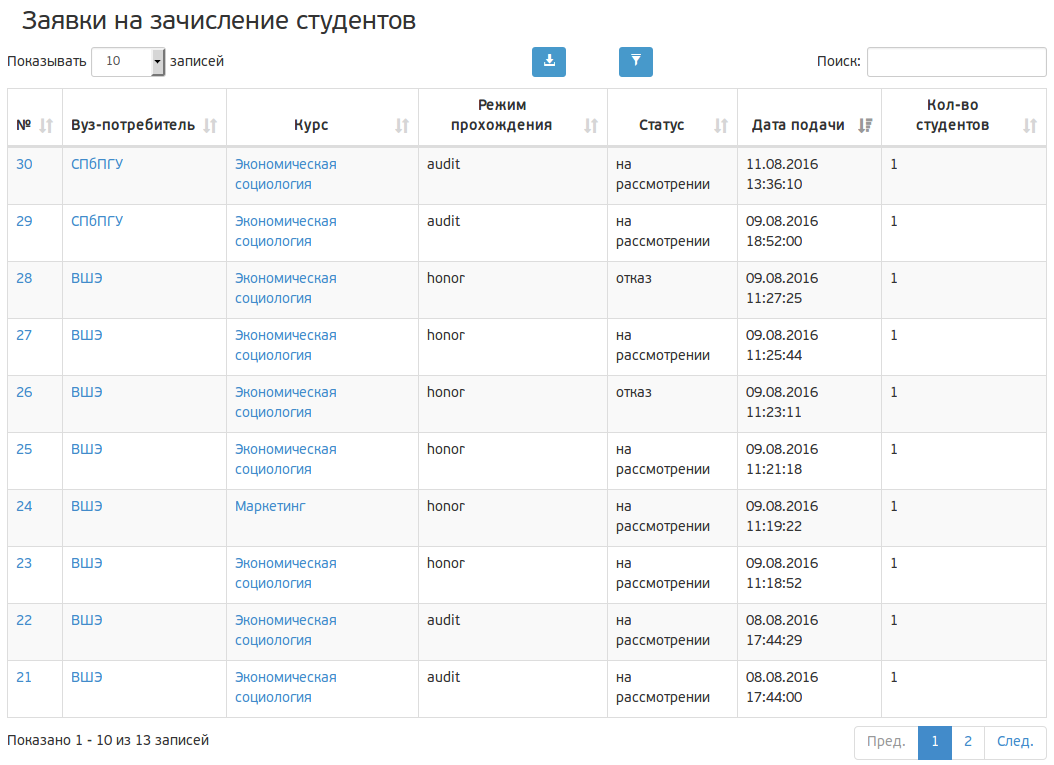
\includegraphics[width=1\linewidth]{enroll_req_list}}
	\caption{Список заявок на зачисление}
	\label{img:agreement:enroll_req_list}
\end{figure}

Таблица содержит следующие столбцы:
\begin{itemize}
	\item Номер заявки;
	\item Вуз-потребитель;
	\item Курс;
	\item Режим прохождения;
	\item Статус;
	\item Дата подачи;
	\item Количество студентов в заявке.
\end{itemize}

 Номер заявки в таблице является ссылкой на страницу просмотра подробной информации о заявке, 
описанной в подразделе~\ref{sec:enroll_req_detail}.

Внешний вид диалога фильтрации списка заявок представлен на рис.~\ref{img:agreement:enroll_req_list_filter}.
Можно фильтровать список по следующим параметрам:
\begin{itemize}
	\item Вуз-потребитель "--- виджет выпадающего списка с автодополнением с возможностью множественного выбора 
	(описание виджета см. в подразделе~\ref{widget:autocomplete_with_multiselect});
	\item Курс "--- виджет выпадающего списка с автодополнением с возможностью множественного выбора 
	(описание виджета см. в подразделе~\ref{widget:autocomplete_with_multiselect});
	\item Режим прохождения "--- виджет выпадающего списка с автодополнением с возможностью множественного выбора 
	(описание виджета см. в подразделе~\ref{widget:autocomplete_with_multiselect});
	\item Статус "--- виджет выпадающего списка с автодополнением с возможностью множественного выбора 
	(описание виджета см. в подразделе~\ref{widget:autocomplete_with_multiselect});
	\item Диапазон дат подачи "--- виджеты выбора даты и времени 
	(описание виджета см. в подразделе~\ref{widget:date_time_picker});
	\item Диапазон количества студентов в заявке "--- числовое поле.
\end{itemize}

\begin{figure}[H]
	\center{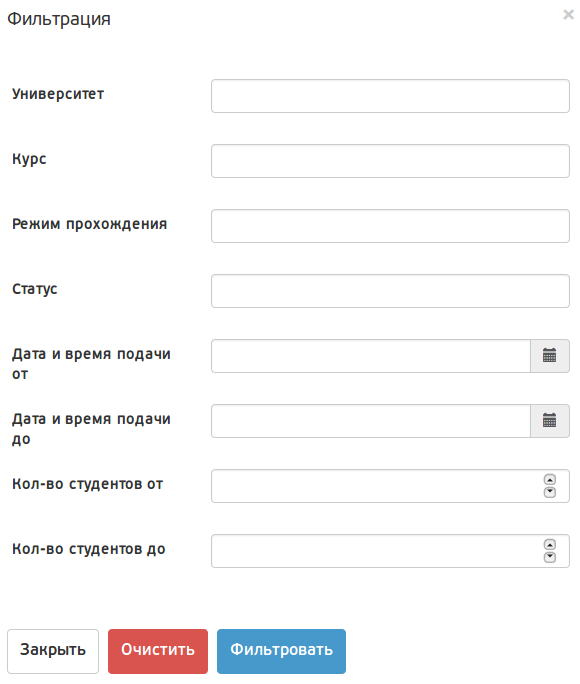
\includegraphics[height=9.1cm]{enroll_req_list_filter}}
	\caption{Диалог фильтрации списка заявок на зачисление}
	\label{img:agreement:enroll_req_list_filter}
\end{figure}

\subsection{Заявки на изменение режима прохождения сессии курса}

Заявки на изменение режима прохождения сессии курса -- это табличное представление заявок на изменение 
режима прохождения сессии курса, полученных данным вузом в качестве вуза-разработчика. 
Элементы управления табличными представления описаны в подразделе~\ref{sec:datatables}.
Внешний вид списка представлен на рис.~\ref{img:agreement:change_mode_req_list}. 

\begin{figure}[H]
	\center{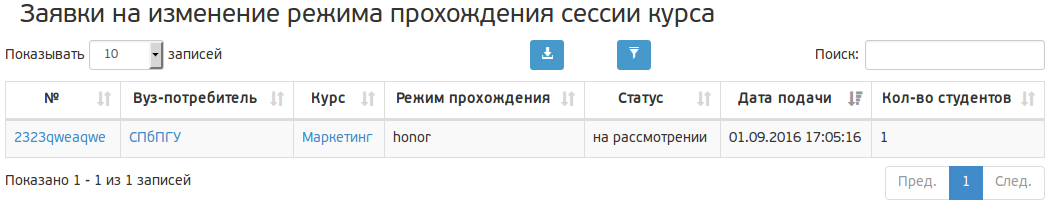
\includegraphics[width=1\linewidth]{change_mode_req_list}}
	\caption{Список заявок на изменение режима прохождения сессии курса}
	\label{img:agreement:change_mode_req_list}
\end{figure}

Таблица содержит следующие столбцы:
\begin{itemize}
	\item Номер заявки;
	\item Вуз-потребитель;
	\item Курс;
	\item Режим прохождения;
	\item Статус;
	\item Дата подачи;
	\item Количество студентов в заявке.
\end{itemize}

Номер заявки в таблице является ссылкой на страницу просмотра подробной информации о заявке, 
описанной в подразделе~\ref{sec:change_mode_req_detail}.

Внешний вид диалога фильтрации списка заявок представлен на рис.~\ref{img:agreement:change_mode_req_list_filter}.
Можно фильтровать список по следующим параметрам:
\begin{itemize}
	\item Вуз-потребитель "--- виджет выпадающего списка с автодополнением с возможностью множественного выбора 
	(см. подраздел~\ref{widget:autocomplete_with_multiselect});
	\item Курс "--- виджет выпадающего списка с автодополнением с возможностью множественного выбора 
	(см. подраздел~\ref{widget:autocomplete_with_multiselect});
	\item Режим прохождения "--- виджет выпадающего списка с автодополнением с возможностью множественного выбора 
	(см. подраздел~\ref{widget:autocomplete_with_multiselect});
	\item Статус "--- виджет выпадающего списка с автодополнением с возможностью множественного выбора 
	(см. подраздел~\ref{widget:autocomplete_with_multiselect});
	\item Диапазон дат подачи "--- виджеты выбора даты и времени 
	(см. подраздел~\ref{widget:date_time_picker});
	\item Диапазон количества студентов в заявке "--- числовое поле.
\end{itemize}

\begin{figure}[H]
	\center{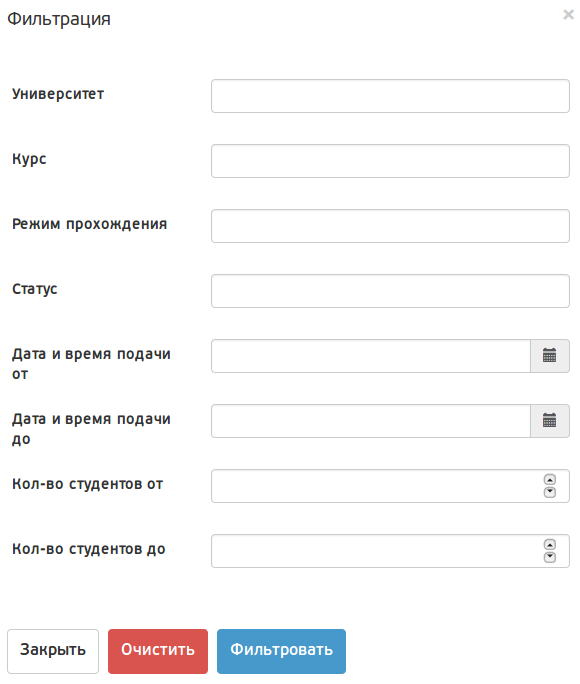
\includegraphics[height=9cm]{enroll_req_list_filter}}
	\caption{Диалог фильтрации списка заявок на изменение режима прохождения сессии курса}
	\label{img:agreement:change_mode_req_list_filter}
\end{figure}

